\documentclass{article}
\usepackage[top=30mm, right=30mm, left=30mm, bottom=30mm]{geometry}
\usepackage[utf8]{vietnam}
\usepackage{amsthm}
\usepackage{amsmath}
\usepackage{amsfonts}
\usepackage{amssymb}
\usepackage{graphicx}
\usepackage{url}
\usepackage{cases}

\title{\textbf{Phân tích thiết kế hệ thống với UML}}
\author{Ngô Quang Dương}
\date{\today}

\begin{document}

\maketitle

\begin{abstract}Trong tài liệu này, mình trình bày một cách ngắn gọn những điều cần biết về việc phân tích thiết kế hệ thống với \textbf{UML} - các loại sơ đồ \textbf{UML}, các giai đoạn trong phân tích thiết kế hệ thống và những việc được thực hiện trong những giai đoạn đó.
\end{abstract}

\tableofcontents

\begin{center}
  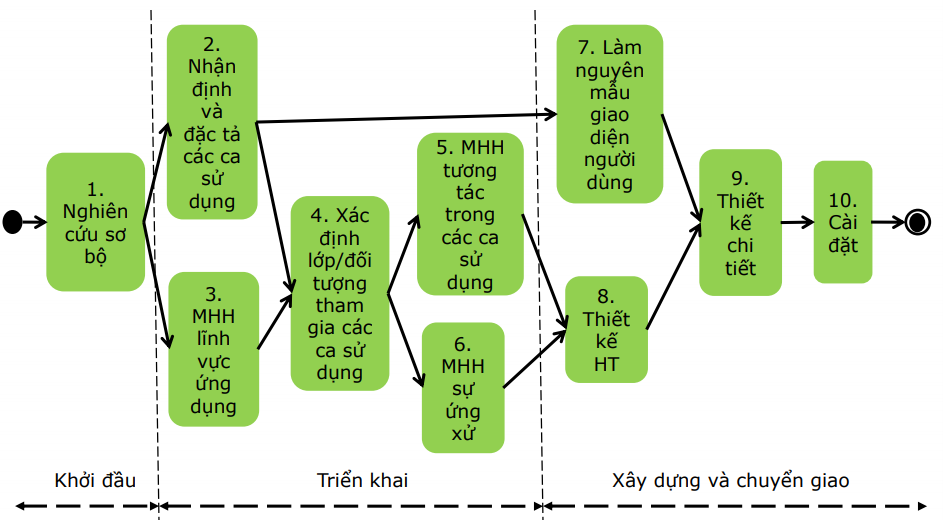
\includegraphics[scale=0.6]{../pictures/rup.PNG}
\end{center}

\section{Các loại sơ đồ}
  
  \subsection{Sơ đồ ca sử dụng}
  
  \paragraph{\textnormal{Thường được gọi nhiều hơn bằng cái tên \textit{sơ đồ use case}, sơ đồ này thể hiện các \textit{tác nhân} hệ thống (là những thành phần có tương tác với hệ thống nhưng không nằm trong hệ thống) và các \textit{chức năng} đối với từng tác nhân.}}

  \paragraph{\textnormal{Trong một \textit{sơ đồ use case} thông thường, các \textit{tác nhân} được biểu diễn bằng hình người que, còn các \textit{chức năng}(use case) được biểu diễn bằng hình elip với nội dung là tên của \textit{chức năng} đó.}}

  Hãy xem qua ví dụ sau:

  \begin{figure}[!ht]
    \centering
    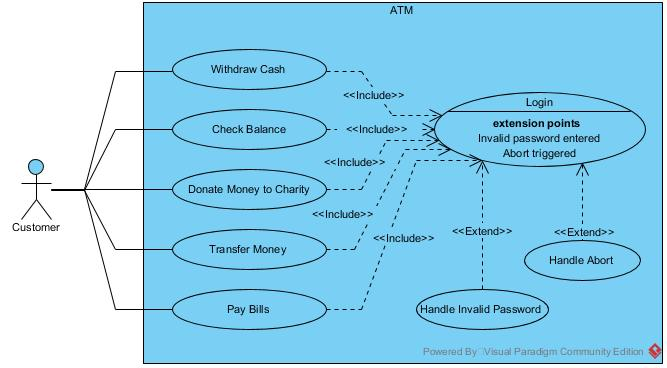
\includegraphics[scale=0.6]{../pictures/diagrams/usecase/usecase-diagram-example.jpg}
    \caption{Sơ đồ use case cho hệ thống ATM}
  \end{figure}

  \paragraph{\textnormal{Giải thích các ký hiệu:}}
  \begin{itemize}
    \item \textit{Khung hình chữ nhật}: đại diện cho hệ thống, cạnh của hình chữ nhật là biên hệ thống, những gì nằm trong là thành phần hệ thống, còn nằm ngoài thì không.
    \item \textit{Người que}: tác nhân.
    \item \textit{Hình elip}: use case.
    \item \textit{Đường nét liền nối người que với hình elip}: thể hiện rằng tác nhân có thể sử dụng use case đó.
    \item \textit{Mũi tên nét đứt với label <<include>>}: thể  hiện rằng use case này(gốc mũi tên) chứa use case kia(ngọn mũi tên).
    \item \textit{Hình elip có extension point}: use case có điểm mở rộng - tức là khi use case đó được thực hiện thì có thể có những tình huống khác xảy ra - như trong sơ đồ trên thì việc đăng nhập có thể đúng hoặc sai, mỗi tình huống đó là một extension point.
    \item \textit{Mũi tên nét đứt với label <<extend>>}: thể hiện rằng use case này(gốc mũi tên) sẽ mở rộng use case kia(ngọn mũi tên), với điều kiện được trình bày trong extension point.
  \end{itemize}

  \subsection{Sơ đồ lớp}

  \paragraph{\textnormal{Sơ đồ lớp (\textit{class diagram}) là sơ đồ thể hiện nội dung của các lớp (thuộc tính, phương thức, bổ từ truy cập) và mối quan hệ giữa các lớp (kế thừa, kết tập, kết hợp, hợp thành).}}

  \begin{figure}[!ht]
    \centering
    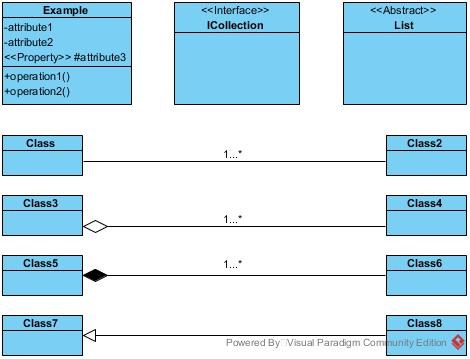
\includegraphics[scale=0.8]{../pictures/diagrams/class/class-diagram-example.jpg}
    \caption{Minh họa các ký hiệu trong sơ đồ lớp}
  \end{figure}

  \paragraph{\textnormal{Giải thích các ký hiệu:}}
  
  \begin{itemize}
    \item \textit{Khung hình chữ nhật}:
      \begin{itemize}
        \item \textit{Khoang trên cùng}: tên class, phần <<...>> trên cùng là stereotype -- để thể hiện những kiểu mà UML không có sẵn như là interface, abstract, \ldots nếu không có gì thì mặc định hiểu đó là class.
        \item \textit{Khoang thứ hai}: danh sách các thuộc tính (có thể bổ sung kiểu dữ liệu).
        \item \textit{Khoang thứ ba}: danh sách các phương thức (có thể bổ sung kiểu dữ liệu trả về và các tham số cùng kiểu dữ liệu tương ứng).
        \item \textit{Dấu -}: \texttt{private}.
        \item \textit{Dấu \#}: \texttt{protected}.
        \item \textit{Dấu +}: \texttt{public}.
      \end{itemize}
      \item \textit{Đường nét liền}: thể hiện quan hệ kết hợp - tức là hai class có tương tác với nhau.
      \item \textit{Đường nét liền có một đầu hình thoi trắng}: thể hiện quan hệ kết tập -- class này(có hình thoi trắng) sở hữu một object của class kia(không có hình thoi trắng) nhưng object của class kia có thể tồn tại độc lập với class này.
      \item \textit{Đường nét liền có một đầu hình thoi đen}: thể hiện quan hệ hợp thành -- cũng tương tự như quan hệ kết tập nhưng khác là object của class kia chỉ tồn tại nếu có object của class này.
      \item \textit{Bội số(1...*, *, 1}: trong mối quan hệ kết hợp với bộ 1 thì object của class bên trái sẽ kết hợp với 1 object của class bên phải; 1...* thì object của class bên trái kết hợp với ít nhất 1 object của class bên phải; * thì object bên trái có thể kết hợp với không hoặc nhiều object của class bên phải.
      \item  \textit{Mũi tên có ngọn hình tam giác trắng}: thể hiện quan hệ tổng quát hóa -- class ở ngọn mũi tên tổng quát class ở gốc mũi tên.
  \end{itemize}

  \subsection{Sơ đồ tuần tự}

  \paragraph{\textnormal{Sơ đồ tuần tự (sequence diagram) được sử dụng để mô tả các thao tác được thực hiện trong một use case -- cụ thể là các object tương tác với nhau như thế nào, gọi tới những phương thức nào.}}

  \paragraph{\textnormal{Các bước của quá trình tương tác rất tiên theo dõi vì chúng được đặt theo thứ tự từ trái sang phải, từ trên xuống dưới và còn được đánh số, sử dụng các mũi tên.}}

  \paragraph{\textnormal{Hãy quan sát sơ đồ tuần tự thể hiện quá trình cho thẻ vào máy ATM :}}

  \begin{figure}[!ht]
    \centering
    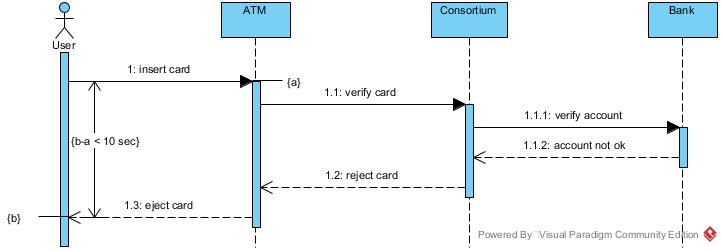
\includegraphics[scale=0.5]{../pictures/diagrams/sequence/sequence-diagram-1.jpg}
    \caption{Sơ đồ tuần tự minh họa việc cho thẻ vào máy ATM}
  \end{figure}

  \paragraph{\textnormal{Giải thích các ký hiệu:}}
  
  \begin{itemize}
    \item \textit{Hình người que}: tác nhân.
    \item \textit{Hình chữ nhật có nhãn}: object.
    \item \textit{Đường nét đứt thẳng}: đường sống (life line).
    \item \textit{Hình chữ nhật dài trên đường sống}: thời gian hoạt động của object hoặc tác nhân đó.
    \item \textit{Mũi tên nét liền}: gọi phương thức của object được trỏ đến.
    \item \textit{Mũi tên nét đứt}: kết quả trả về.
  \end{itemize}

  \paragraph{\textnormal{Có thể thấy rằng thứ tự được gọi của các phương thức được thể hiện qua cách đánh số và cách sắp xếp từ trái sang phải, từ trên xuống dưới.
  }}

  \begin{figure}[!ht]
    \centering
    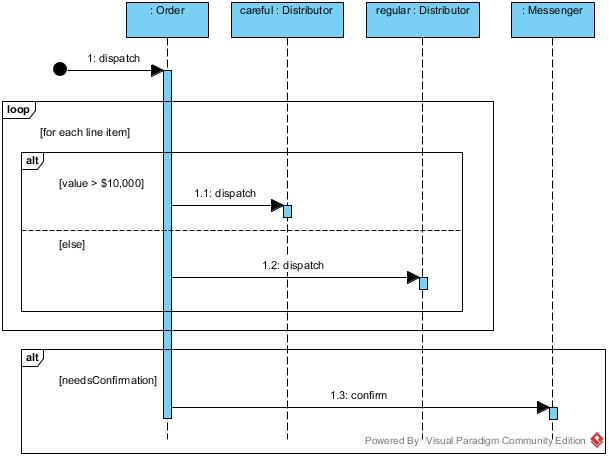
\includegraphics[scale=0.5]{../pictures/diagrams/sequence/sequence-diagram-2.jpg}
    \caption{Ví dụ về cấu trúc lặp và rẽ nhánh trong sơ đồ tuần tự}
  \end{figure}

  Ngoài ra, trong sơ đồ tuần tự, người ta còn có thể trình bày các cấu trúc lặp, rẽ nhánh, \texttt{continue}, \texttt{break}. Trong đó, cấu trúc lặp, rẽ nhánh sẽ được đặt vào một khung có nhãn lần lượt là \textbf{loop} và \textbf{alt}.

  \subsection{Sơ đồ giao tiếp}

  \paragraph{\textnormal{Sơ đồ giao tiếp(communication diagram) có tác dụng giống hệt như sơ đồ tuần tự. Ưu điểm của nó so với sơ đồ tuần tự là sơ đồ giao tiếp có thể trình bày tự do hơn, trong khi sơ đồ tuần tự có một cấu trúc cố định (sẽ càng chiếm nhiều diện tích hơn khi số lượng object hoặc các bước tăng lên). Nhược điểm là nó không tiện theo dõi thứ tự các bước như trong sơ đồ tuần tự.}}

  \begin{figure}[!ht]
    \centering
    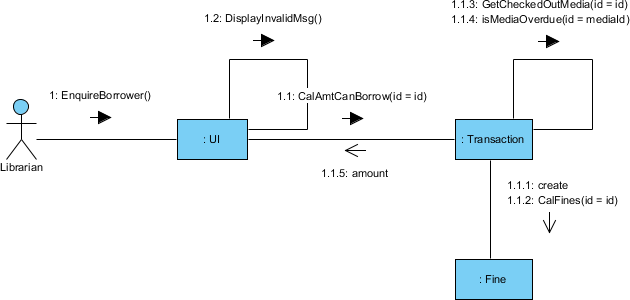
\includegraphics[scale=0.7]{../pictures/diagrams/communication/communication-diagram-1.png}
    \caption{Sơ đồ giao tiếp thể hiện quá trình mượn sách}
  \end{figure}


  \subsection{Sơ đồ hoạt động}

  \paragraph{\textnormal{
    Sơ đồ hoạt động(activity diagram) khá giống với sơ đồ luồng, sơ đồ khối (flowchart). Nếu như sơ đồ tuần tự và sơ đồ giao tiếp thể hiện các object và lời gọi các phương thức thì ở sơ đồ hoạt động, quá trình đó được thể hiện chi tiết hơn -- có thể hiểu là sơ đồ này sẽ trình bày cả những điều được thực hiện bên trong phương thức.
  }}

  \paragraph{\textnormal{
    Sơ đồ hoạt động luôn bắt đầu bằng một node bắt đầu (một hình tròn đen) và đích đến là node kết thúc (hình tròn đen có viền). Một sơ đồ hoạt động luôn có đúng một node bắt đầu nhưng có thể có nhiều node kết thúc (tương ứng với nhiều tình huống khác nhau).
  }}

  \paragraph{\textnormal{
    Các bước của một quá trình được thể hiện trong sơ đồ hoạt động bằng các hình chữ nhật có bo tròn góc. Các mũi tên sẽ trỏ luồng hoạt động. Cũng giống như trong sơ đồ khối, sơ đồ hoạt động cũng có thể thể hiện cấu trúc rẽ nhánh (bằng node quyết định hình thoi) và cấu trúc lặp.
  }}

  \begin{figure}[!ht]
    \centering
    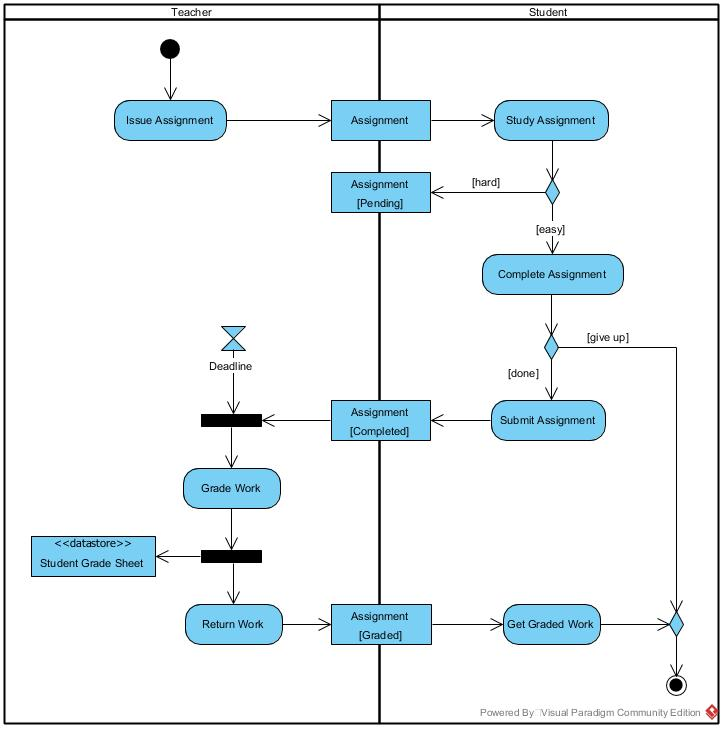
\includegraphics[scale=0.4]{../pictures/diagrams/activity/activity-diagram-1.jpg}
    \caption{Sơ đồ hoạt động}
  \end{figure}

  \subsection{Sơ đồ máy trạng thái}

  \paragraph{\textnormal{
    Trong lập trình hướng đối tượng, một đối tượng có hai đặc tính: thứ nhất là thuộc tính(property or attribute), thứ hai là phương thức(method or operation). Trong đó, thuộc tính cũng chính là \textit{trạng thái} của đối tượng.
  }}
  \paragraph{\textnormal{
    Sơ đồ máy trạng thái(state machine diagram) chỉ ra trạng thái của hệ thống và những sự kiện, phương thức có thể kích hoạt sự thay đổi của những thuộc tính đó.
  }}

  \begin{figure}[!ht]
    \centering
    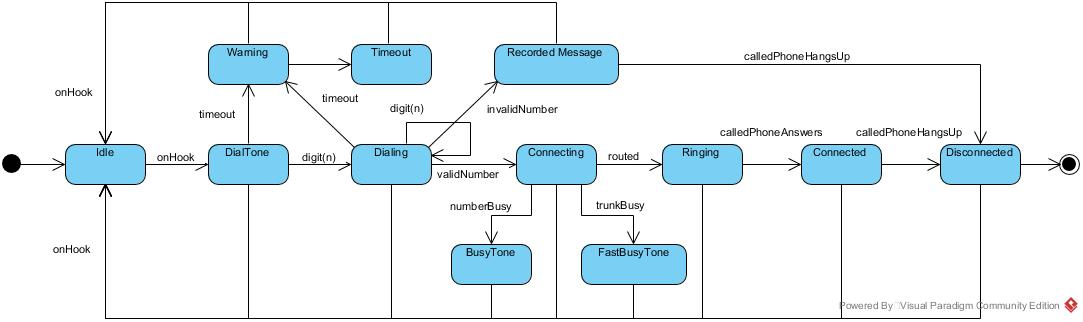
\includegraphics[scale=0.4]{../pictures/diagrams/statemachine/state-machine-diagram-1.jpg}
    \caption{Minh họa sơ đồ máy trạng thái cho hệ thống điện thoại}
  \end{figure}

  \subsection{Sơ đồ quan hệ thực thể}

  \paragraph{\textnormal{
    Sơ đồ quan hệ thực thể(entity relationship diagram) thể hiện mối quan hệ giữa các thực thể được lưu trữ trong một cơ sở dữ liệu. Thực thể trong ngữ cảnh này chính là những object. Một tập thực thể là một bộ các thực thể cùng loại. Các thực thể có thể có một hoặc nhiều thuộc tính.
  }}

  \paragraph{\textnormal{
    Mối quan hệ trong sơ đồ quan hệ thực thể có thể thuộc một trong các loại sau, còn được gọi là những bội số. Bội số nếu có thể nhận giá trị $0$ được gọi là \textit{optional}(tùy chọn), ngược lại được gọi là \textit{mandatory}(bắt buộc).
  }}

  \begin{itemize}
    \item \textbf{1 -- 1}. Quan hệ một -- một, được thể hiện bằng đường nối:
    \begin{figure}[!ht]
      \centering
      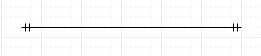
\includegraphics[scale=1]{../pictures/diagrams/entityrelationship/1to1.PNG}
      \caption{1 -- 1}
    \end{figure}
    \begin{figure}[!ht]
      \centering
      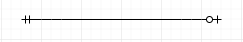
\includegraphics[scale=1]{../pictures/diagrams/entityrelationship/1-mandatory-to-1-optional.PNG}
      \caption{1 -- 0\ldots 1}
    \end{figure}
    \item \textbf{1 -- n}. Quan hệ một -- nhiều:
    \begin{figure}[!ht]
      \centering
      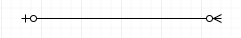
\includegraphics[scale=1]{../pictures/diagrams/entityrelationship/1-optional-to-Many-optional.PNG}
      \caption{0..1 -- 0..n}
    \end{figure}
    \begin{figure}[!ht]
      \centering
      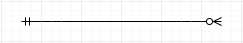
\includegraphics[scale=1]{../pictures/diagrams/entityrelationship/1-mandatory-to-Many-optional.PNG}
      \caption{1 -- 0..n}
    \end{figure}
    \begin{figure}[!ht]
      \centering
      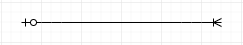
\includegraphics[scale=1]{../pictures/diagrams/entityrelationship/1-optional-to-Many-mandatory.PNG}
      \caption{0..1 -- n}
    \end{figure}
    \begin{figure}[!ht]
      \centering
      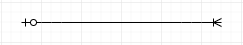
\includegraphics[scale=1]{../pictures/diagrams/entityrelationship/1-optional-to-Many-mandatory.PNG}
      \caption{1 -- n}
    \end{figure}
    \item \textbf{n -- n}. Quan hệ nhiều -- nhiều:
    \begin{figure}[!ht]
      \centering
      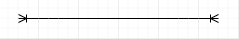
\includegraphics[scale=1]{../pictures/diagrams/entityrelationship/Many-mandatory-to-Many-mandatory.PNG}
      \caption{n -- n}
    \end{figure}
    \begin{figure}[!ht]
      \centering
      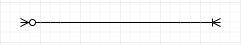
\includegraphics[scale=1]{../pictures/diagrams/entityrelationship/Many-optional-to-Many-mandatory.PNG}
      \caption{0..n -- n}
    \end{figure}
    \begin{figure}[!ht]
      \centering
      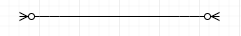
\includegraphics[scale=1]{../pictures/diagrams/entityrelationship/Many-optional-to-Many-optional.PNG}
      \caption{0..n -- 0..n}
    \end{figure}
  \end{itemize}

  \begin{figure}[!ht]
    \centering
    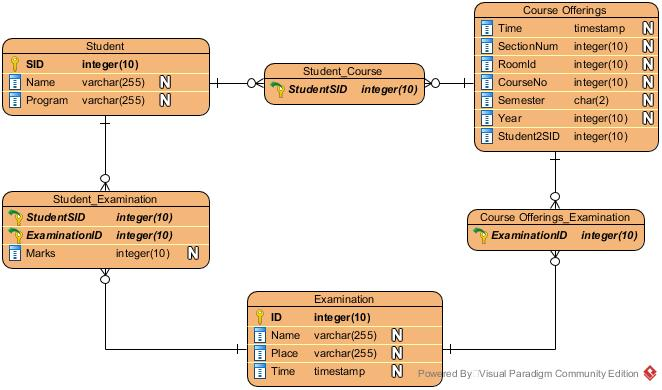
\includegraphics[scale=0.5]{../pictures/diagrams/entityrelationship/entity-relationship-diagram-1.jpg}
    \caption{Ví dụ sơ đồ quan hệ thực thể cho cơ sở dữ liệu lưu trữ điểm của sinh viên}
  \end{figure}

  \subsection{Sơ đồ gói}

  \paragraph{\textnormal{
    Một tính chất khác của lập trình hướng đối tượng là tính đóng gói. Có hai khía cạnh của tính đóng gói: thứ nhất là sự giới hạn truy cập một thuộc tính, phương thức của đối tượng; thứ hai là sự nhóm họp của các class có cùng chức năng. Khía cạnh thứ nhất đã được thể hiện trong \textit{sơ đồ lớp}, còn khía cạnh thứ hai được thể hiện trong sơ đồ gói(package diagram)
  }}

  \begin{figure}[!ht]
    \centering
    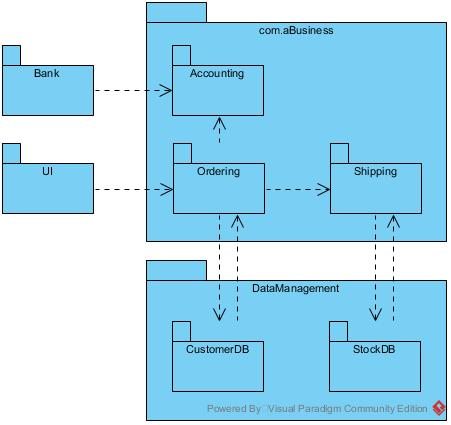
\includegraphics[scale=0.5]{../pictures/diagrams/package/package-diagram-1.jpg}
    \caption{Sơ đồ gói}
  \end{figure}

  \paragraph{\textnormal{
    Giải thích các ký hiệu:
  }}

  \begin{itemize}
    \item \textit{Hình tập tài liệu}: đại diện cho một package, các package có thể rời nhau hoặc package này chứa một hay nhiều package con.
    \item \textit{Mũi tên nét đứt}: quan hệ phụ thuộc, package ở gốc mũi tên phụ thuộc vào package ở ngọn mũi tên.
  \end{itemize}

  \paragraph{\textnormal{
    Ngoài ra trong các package trên sơ đồ gói có thể biểu diễn thêm các class, interface bên trong.
  }}

  \subsection{Sơ đồ triển khai}

  \paragraph{\textnormal{
    Sơ đồ triển khai (deployment diagram) được sử dụng để mô tả sự bố trí các \textit{thành phần thực thi}.
  }}

  \paragraph{\textnormal{
    Các thành phần đó có thể là phần cứng(nút cứng, các thiết bị vật lý, \ldots) hoặc phần mềm(nút mềm, các file thực thi, server, \ldots). Các nút trong một sơ đồ triển khai được kết nối với nhau.
  }}

  \begin{figure}[!ht]
    \centering
    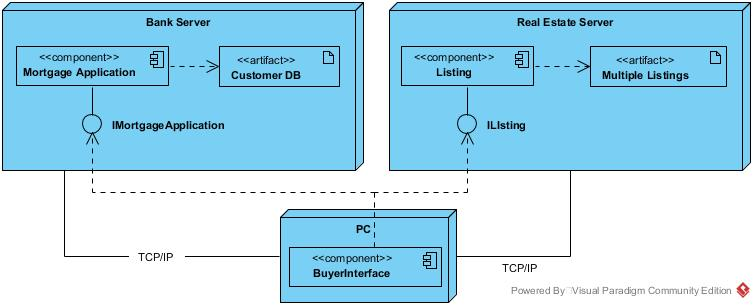
\includegraphics[scale=0.5]{../pictures/diagrams/deployment/deployment-diagram-1.jpg}
    \caption{Sơ đồ triển khai}
  \end{figure}

  \paragraph{\textnormal{
    Giải thích các ký hiệu:
  }}
  \begin{itemize}
    \item \textit{Hình hộp}: một nút.
    \item \textit{Các stereotype}: các thành phần trong một nút.
    \item \textit{Hình tròn}: giao diện(interface).
    \item \textit{Mũi tên nét đứt}: thể hiện việc sử dụng, cài đặt giao diện.
  \end{itemize}

\section{Các giai đoạn trong phân tích thiết kế}

  \subsection{Phân tích yêu cầu}

  \subsection{Đặc tả yêu cầu}

  \subsection{Xác định các class/object phân tích}

  \subsection{Mô tả quá trình tương tác trong một use case}

  \subsection{Thiết kế hệ thống con}

  \subsection{Lựa chọn công nghệ}

  \subsection{Cài đặt và triển khai}

\end{document}
